%% Modified from the Use Cases Template File:

%% Created by Tom Desair (http://www.tomdesair.com)
%% Downloadable at: http://www.tomdesair.com/downloads/use-case-latex-template.zip
%% Date Modified: 03/04/2012
%
% This work may be distributed and/or modified under the
% conditions of the LaTeX Project Public License, either version 1.3
% of this license or (at your option) any later version.
% The latest version of this license is in
%   http://www.latex-project.org/lppl.txt
% and version 1.3 or later is part of all distributions of LaTeX
% version 2005/12/01 or later.

\documentclass[a4paper, 10pt, oneside, draft]{article}

\usepackage[utf8]{inputenc}
\usepackage{usecases}
\usepackage{enumerate}
\usepackage[final]{graphicx}
\graphicspath{ {../uml/} }
\title{Library Project Requirements Analysis Document}
\date{\today}
\author{Adam Kimball, Alex Macri, Corey Richardson}

\begin{document}

\maketitle
\newpage

\tableofcontents
\newpage

\section{Preliminary Report}

After further meeting and consideration, our team has come to the conclusion that the majority of the
initially established directives are going to be implemented within the finished product, as they line
up directly with the needs of the Clarkson Open Source Institute. The intended feature list can be broken
into a series of use cases, as will be demonstrated below.

The first portion of the project consists of a library management system, described by the following use
cases:

\begin{itemize}
	\item As a library maintainer, I want a database of every book currently owned by the COSI library.
	\item As a library maintainer, I want to be able to restrict certain books from being checked out by students.
	\item As a library maintainer, I want to beable to keep tabsonwho has what book, and for how long.
	\item As a user of the library, I want to be capable of checking out books without needing to notify the library maintainer
	\item As a user of the library, I want to be able into check out books without requiring any non-standard identification upon loan
	\item As a user of the library, I want to be able to check out books conveniently, without having to type in book information each time I wish to check out.
	\item As a user of the library, I want like to have a web interface for keeping track of which books I currently have on loan, and which books are
available for loan.
	\item As a user of the library, I want this web interface to provide information on the books available to me.
\end{itemize}

Additionally, while not considered a requirement for completion, there are several use cases whose implementation are desirable for the labs' frequent members:

\begin{itemize}
	\item As a member of the Clarkson Open Source Institute, I want to be able to access a web service to view any recorded meetings I may have missed.
	\item As a member of the Clarkson Open Source Institute, I want to be able to view any transcripts/meeting minutes that have been written on the same page as the video.
	\item As the secretary of the Clarkson Open Source Institute, I want to have a means of uploading video recordings of the meetings, and submit accompanying transcripts/meeting minutes.
	\item As the secretary of the Clarkson Open Source Institute, I want to upload chat logs/email threads that are viewable/searchable by members of the labs.
	\item As the secretary of the Clarkson Open Source Institute, I want to be able to edit this information with a plain text editor, without needing to learn non-standard version control systems.
\end{itemize}

We are also considering the idea of using the Wiki to provide a couple of other services, but details of this have not yet been worked out.

The workload for out group is going to be divided as follows:

\begin{itemize}
	\item Adam Kimball
		\begin{itemize}
 			\item Writing and refining the web front-end for users to access
		\end{itemize}
	\item Corey Richardson
		\begin{itemize}
			\item Construction and implementation of the scanning machine for users to manage
				book check-in/check-out
		\end{itemize}
	\item Alex Macri
		\begin{itemize}
			\item Creation and initial maintainence of the book database, and implementing
				an easy way for library maintainers to make changes to the database.
		\end{itemize}
\end{itemize}

\newpage

\section{Use Cases}

%Sometimes it is a good idea to put domain objects in \texttt{}
%The template and the descriptions are based on the book Applying UML and Patterns:
%An Introduction to Object-Oriented Analysis and Design and Iterative Development
%(3rd Edition) by Craig Larman.
\begin{usecase}

\addtitle{Use Case 1}{Handle Book Checkout \textit{(Corey Richardson)}}

%Scope: the system under design
\addfield{Scope:}{Library Management System}

%Level: "user-goal" or "subfunction"
\addfield{Level:}{User-goal}

%Primary Actor: Calls on the system to deliver its services.
\addfield{Primary Actor:}{Lab Member}

%Stakeholders and Interests: Who cares about this use case and what do they want?
\additemizedfield{Stakeholders and Interests:}{
	\item Lab Member: Wants to check out books easily, using student ID card,
        and without entering book information manually.
    \item Library Maintainer: Wants certain books to not be checked out, and
        users to only be able to checkout a certain number of books.
}

%Preconditions: What must be true on start and worth telling the reader?
%\addfield{Preconditions:}{}
%when multiple
\additemizedfield{Preconditions:}{
    \item Lab Member must have a valid student ID.
    \item Book must be in the library (cannot check out book online).
    \item Library barcode scanner is present and functional.
}

%Postconditions: What must be true on successful completion and worth telling the reader
%\addfield{Postconditions:}{}
%when multiple
\additemizedfield{Postconditions:}{
    \item Book is assigned to the user.
    \item The user's quota is decremented.
    \item The book is marked as ``unavailable''.
}

%Main Success Scenario: A typical, unconditional happy path scenario of success.
\addscenario{Main Success Scenario:}{
	\item The user browses the bookshelves.
    \item The user takes the book to the scanner.
    \item \label{itm:scancommand} The user scans the ``checkout book'' command on a command sheet.
    \item \label{itm:scanid} The user scans their student ID barcode.
    \item \label{itm:scanbarcode} The user scans the book's barcode.
    \item The scanner makes a ``success'' beep, indicating
        that the user has successfully checked out the book.
}

%Extensions: Alternate scenarios of success or failure.
\addscenario{Extensions:}{
    \item[\ref{itm:scancommand}a.] Invalid command:
        \begin{enumerate}[1.]
		\item Scanner makes a ``failure'' beep, and uses text-to-speech to
            state ``Invalid Command''.
        \item User returns to step \ref{itm:scancommand} and re-scans a
            correct command.
		\end{enumerate}

    \item[\ref{itm:scanid}a.] Unknown ID:
        \begin{enumerate}[1.]
        \item Scanner makes a ``failure'' beep, and uses text-to-speech to
            state ``Unknown ID''.
        \item User registers their ID (see ``Registration'' usecase)
        \end{enumerate}

    \item[\ref{itm:scanbarcode}a.] Unknown ISBN:
        \begin{enumerate}[1.]
        \item Scanner sends ISBN to server to register it as part of the
            library, followed by a checkout command.
        \item Server fetches the book information and adds it to the library
            database, as well as checking out that book to the user.
        \item Scanner makes a ``success'' beep.
        \end{enumerate}

    \item[\ref{itm:scanbarcode}b.] Book already checked out:
        \begin{enumerate}[1.]
        \item Scanner uses tex-to-speech to state ``Book checked out to (User
            Currently Assigned To Book), add new copy?''.
        \item User scans ``Yes'' or ``No'' command from command sheet.
        \item If Yes, server adds another copy of that book to the library and
            checks it out to the user.
        \item If No, prompt the user whether the book should be checked out.
            \begin{enumerate}[1.]
            \item If Yes, check the book out from the other user.
            \item If No, emit ``failure'' beep and use text-to-speech to state
                ``Already checked out, ask (User Currently Assigned To Book)
                to check it out''.
            \end{enumerate}
        \end{enumerate}
}

%Special Requirements: Related non-functional requirements.
\additemizedfield{Special Requirements:}{
	\item Scanner responds within 1 second 90\% of the time.
	\item Scanner resets all commands after 1 minute of waiting for input, to
        handle users walking away.
}

%Technology and Data Variations List: Varying I/O methods and data formats.
\addscenario{Technology and Data Variations List:}{
	\item All interaction done with a barcode scanner using standard user ID
        cards and ISBN barcodes.
}

%Frequency of Occurrence: Influences investigation, testing and timing of implementation.
\addfield{Frequency of Occurrence:}{Multiple times per week.}

%Miscellaneous: Such as open issues/questions
%\addfield{Open Issues:}{}

\end{usecase}


%new usecase

\newpage

\begin{usecase}


\addtitle{Use Case 2}{Handle User Book Checkin \textit{(Corey Richardson)}}
\addfield{Scope:}{Library Management System}
\addfield{Level:}{User-goal}
\addfield{Primary Actor:}{End-user}
\additemizedfield{Stakeholders and Interests:}{
    \item Lab Member: Wants to easily return a previously checked-out book.
}

\addscenario{Main Success Scenario:}{
    \item User scans ``Check In'' command.
    \item User scans user ID (this is to handle multiple copies of a book
        being signed out to multiple users).
    \item User scans book barcode.
    \item Scanner emits ``success'' beep to indicate successful completion.
}

\end{usecase}

\newpage

\begin{usecase}

\addtitle{Use Case 3}{Handle User Searching for Books \textit{(Adam Kimball)}}

%Scope: the system under design
\addfield{Scope:}{Library Management System}

%Level: "user-goal" or "subfunction"
\addfield{Level:}{User-goal}

%Primary Actor: Calls on the system to deliver its services.
\addfield{Primary Actor:}{End-user}

%Stakeholders and Interests: Who cares about this use case and what do they want?
\additemizedfield{Stakeholders and Interests:}{
	\item Lab Member: Wants to easily find a list of books presently available for checkout, with descriptions for each.
	\item Library Maintainer: Wants to have a list available without manually keeping track of each book, or having to inform Lab Members of the book's status.
}

%Preconditions: What must be true on start and worth telling the reader?
%\addfield{Preconditions:}{}
%when multiple
\additemizedfield{Preconditions:}{
	\item System is functional.
	\item System is populated with books.
}

%Postconditions: What must be true on successful completion and worth telling the reader
%\addfield{Postconditions:}{User has been served a list of books relevant to input}
%when multiple
\additemizedfield{Postconditions:}{
	\item User has been served a list of relevant books, if any exist.
	\item User has been given an empty list, if there are no books relevant to input.
}

%Main Success Scenario: A typical, unconditional happy path scenario of success.
\addscenario{Main Success Scenario:}{
	\item \label{itm:webpage} User visits the Library webpage.
	\item \label{itm:search} User types a book title or author into text field, and clicks 'search'.
	\item \label{itm:listing} User is returned a paginated list of all books containing that text in their title or author name, with a truncated version of their description for each, and whether or not each is available for loan.
}

%Extensions: Alternate scenarios of success or failure.
\addscenario{Extensions:}{
	\item[\ref{itm:search}a.] User selects 'All Books' link, rather than inputting a search term:
		\begin{enumerate}[1.]
		\item User selects 'All Books'.
		\item User is presented with a paginated listing of all books from the book database, a truncated version of their description, and whether or not they are available for loan.
		\end{enumerate}
	\item[\ref{itm:listing}a.]User selects a book:
		\begin{enumerate}[1.]
		\item User clicks on a book in the list.
		\item User is redirected to a page with large cover image(if available), and a full description.
		\end{enumerate}
	\item[\ref{itm:listing}b.] User does not input a search that has a result:
		\begin{enumerate}[1.]
		\item No books or authors match user's search.
		\item User is returned an empty list.
		\end{enumerate}
}

%Special Requirements: Related non-functional requirements.
\additemizedfield{Special Requirements:}{
	\item Search results returned by server within 5 seconds 90\% of the time.
	\item Books with no available cover image have an implemented placeholder image.
	\item List served is clean/easy to read.
}

%Technology and Data Variations List: Varying I/O methods and data formats.
\additemizedfield{Technology and Data Variations List:}{
	\item Accessible with recent versions of IE, Chrome, Firefox, and text-based browsers such as Lynx/Elinks.
}
%Frequency of Occurrence: Influences investigation, testing and timing of implementation.
\addfield{Frequency of Occurrence:}{Multiple times per week.}

%Miscellaneous: Such as open issues/questions
%\addfield{Open Issues:}{}

\end{usecase}

\newpage


\begin{usecase}

\addtitle{Use Case 4}{Viewing Meeting Videos \textit{(Adam Kimball)}}
\addfield{Scope:}{Clarkson Open Source Institute Wiki}
\addfield{Level:}{User-goal}
\addfield{Primary Actor:}{End-user}
\additemizedfield{Stakeholders and Interests:}{
    \item Lab Member: Wants to easily view recorded lab meetings or meeting minutes they may have missed.
}

\addscenario{Main Success Scenario:}{
    \item User accesses video portion of the COSI Wiki site.
    \item User selects a meeting date
    \item User is presented with an embedded video player, as well as a small
        summary of what happened at the meeting
}

\end{usecase}


\newpage


\begin{usecase}

\addtitle{Use Case 5}{Interfacing with Database \textit{(Alex Macri)}}

%Scope: the system under design
\addfield{Scope:}{Library Management System}

%Level: "user-goal" or "subfunction"
\addfield{Level:}{User-goal}

%Primary Actor: Calls on the system to deliver its services.
\addfield{Primary Actor:}{Scanner and Web Interface}

%Stakeholders and Interests: Who cares about this use case and what do they want?
\additemizedfield{Stakeholders and Interests:}{
	\item  User:
	Wants to easily find a book with the description and if the book is checkout and if the book is checkout when will the be returned.
	See valuable information in a timely fashion.
	Usable functionality of the database so it is easy to use, understand, and works as expected.
	\item Maintainer:
	For modularity so it is easier to add more functions when needed in the future.
	The database to be fast with searching through the list of books.
}

%Preconditions: What must be true on start and worth telling the reader?
%\addfield{Preconditions:}{}
%when multiple
\additemizedfield{Preconditions:}{
	\item System is functional.
	\item System is populated with books.
	\item System has functionality for user requests from the browser.
}

%Postconditions: What must be true on successful completion and worth telling the reader
%\addfield{Postconditions:}{\textit{None}}
%when multiple
\additemizedfield{Postconditions:}{
    \item The Database preforms all tasks correctly
    \item When requested to list the books. The System will return the either error or on success return the list in a proper format.
    \item When requested to add a book. The System with add the book with the correct information for the book.
    \item When requested to delete a book. The System with delete the book with the correct information for the book.
    \item When requested to checkout and checkin a book. The System with a flag on whether the book is checked-in or checked-out the book with the correct information for the book.

}

%Main Success Scenario: A typical, unconditional happy path scenario of success.
\addscenario{Main Success Scenario:}{
	\item User visits the Library webpage.
	\item User selects a function that with interact with the database.
	\item User is presented functionality of these procedures and can complete the task required.
	\item User completes functionality of the database in 1 sec.
}

%Extensions: Alternate scenarios of success or failure.
\addscenario{Extensions:}{
	\item[1a.] Invalid login data:
        \begin{enumerate}[1.]
		\item System shows failure message.
		\item User cannot login and prompts the user to retry.
		\end{enumerate}
	\item[1b.] Valid login data:
        \begin{enumerate}[1.]
		\item System shows success message.
		\item User continues onto the site.
		\end{enumerate}
	\item[2a.] Invalid checkout data:
        \begin{enumerate}[1.]
		\item[1.] System shows failure message.
		\end{enumerate}
	\item[2b.] Valid checkout data:
        \begin{enumerate}[1.]
		\item System shows success message.
		\item User has checked out out the book and the database is modified.
		\end{enumerate}
	\item[3a.] Invalid checkin data:
        \begin{enumerate}[1.]
		\item System shows failure message.
		\end{enumerate}
	\item[3b.] Valid checkin data:
        \begin{enumerate}[1.]
		\item System shows success message.
		\item User has checked in out the book and the database is modified.
		\end{enumerate}
	\item[4a.] Invalid delete data:
        \begin{enumerate}[1.]
		\item System shows failure message.
		\end{enumerate}
	\item[4b.] Valid delete data:
        \begin{enumerate}[1.]
		\item System shows success message
		\item User updates the database with the book entry gone.
		\end{enumerate}
	\item[5a.] Invalid add data:
        \begin{enumerate}[1.]
		\item System shows failure message.
		\end{enumerate}
	\item[5b.] Valid add data:
        \begin{enumerate}[1.]
		\item System shows failure message.
		\item User adds a book to the database.
		\end{enumerate}
	\item[6a.] Invalid list data:
        \begin{enumerate}[1.]
		\item System shows failure message.
		\end{enumerate}
	\item[6b.] Valid list data:
        \begin{enumerate}[1.]
		\item System shows success message.
		\item User list the books that are currently in the database.
		\end{enumerate}
}

%Special Requirements: Related non-functional requirements.
\additemizedfield{Special Requirements:}{
	\item Response to request in a fast and reasonable timeframe.
}

%Technology and Data Variations List: Varying I/O methods and data formats.
\addscenario{Technology and Data Variations List:}{
	\item Implemented with the Rust programming language.
	\item Uses PostgreSQL database server.
	\item Runs on standard Linux systems.
}

%Frequency of Occurrence: Influences investigation, testing and timing of implementation.
\addfield{Frequency of Occurrence:}{
	Multiple time per week.
}

%Miscellaneous: Such as open issues/questions
%\addfield{Open Issues:}{}

\end{usecase}
\newpage

\begin{usecase}

\addtitle{Use Case 6}{Loading from Database \textit{(Alex Macri)}}
\addfield{Scope:}{Library Management System}
\addfield{Level:}{User-goal}
\addfield{Primary Actor:}{User of System}
\additemizedfield{Stakeholders and Interests:}{
    \item Lab Member: Wants to easily be able to query checked-in or checked-out books.
    \item Lab Member: Wants to easily change the check in and check out status.
}

\addscenario{Main Success Scenario:}{
    \item System gets the request and changes the flag for the book specified or returns error if invalid book
    \item System return success message if the procedure in successful
}

\end{usecase}

\newpage

\section{Design Goals}

The following design goals have been identified:

\begin{itemize}
    \item \textit{Ease of adding new books to the library.} The whole purpose
        of this software system is to achieve this goal, to ensure that the
        lab's library is well maintained into the future. This leads to the
        amount of steps for adding books being as minimal as possible,
        requiring no typing and using existing bar codes.
    \item \textit{Ease of finding existing books.} The system needs to be
        applicable to more than just the library maintainer. The search and
        browsing features of the website work to accomplish this goal. It is
        conceivable that more ways of accessing this information may be
        desired in the future.
    \item \textit{High availability.} The library is used frequently and at
        all times of the day. Therefore, the library administration system
        should have minimal unscheduled downtime.
    \item \textit{Uses available computing resources in the COSI server room.}
        This is a practical non-functional requirement imposed by the client.
        The library management system should integrate with the existing
        infrastructure as much as possible, for ease of administration.
    \item \textit{Uses a comprehensible architecture for future maintainers.}
        After this system is designed and implemented, further requirements
        may come to light as the system is used and the library's needs grow.
        Further developers need to be able to understand and modify the
        system, fixing bugs and adding features as necessary.
\end{itemize}

\newpage

\section{Diagrams}

\begin{figure}[p]
    \centering
    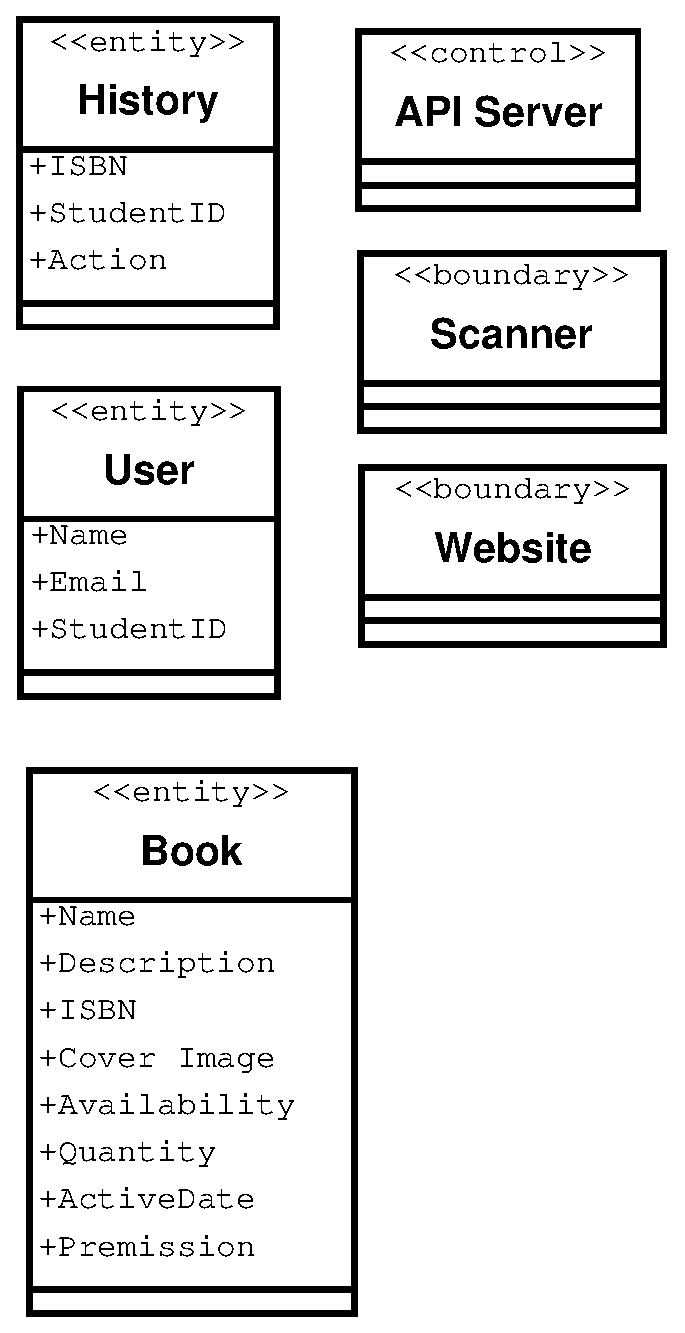
\includegraphics[width=0.9\textwidth]{Objects.eps}
    \caption{Object Diagrams}
    \label{fig:objects_image}
\end{figure}

\begin{figure}[p]
    \centering
    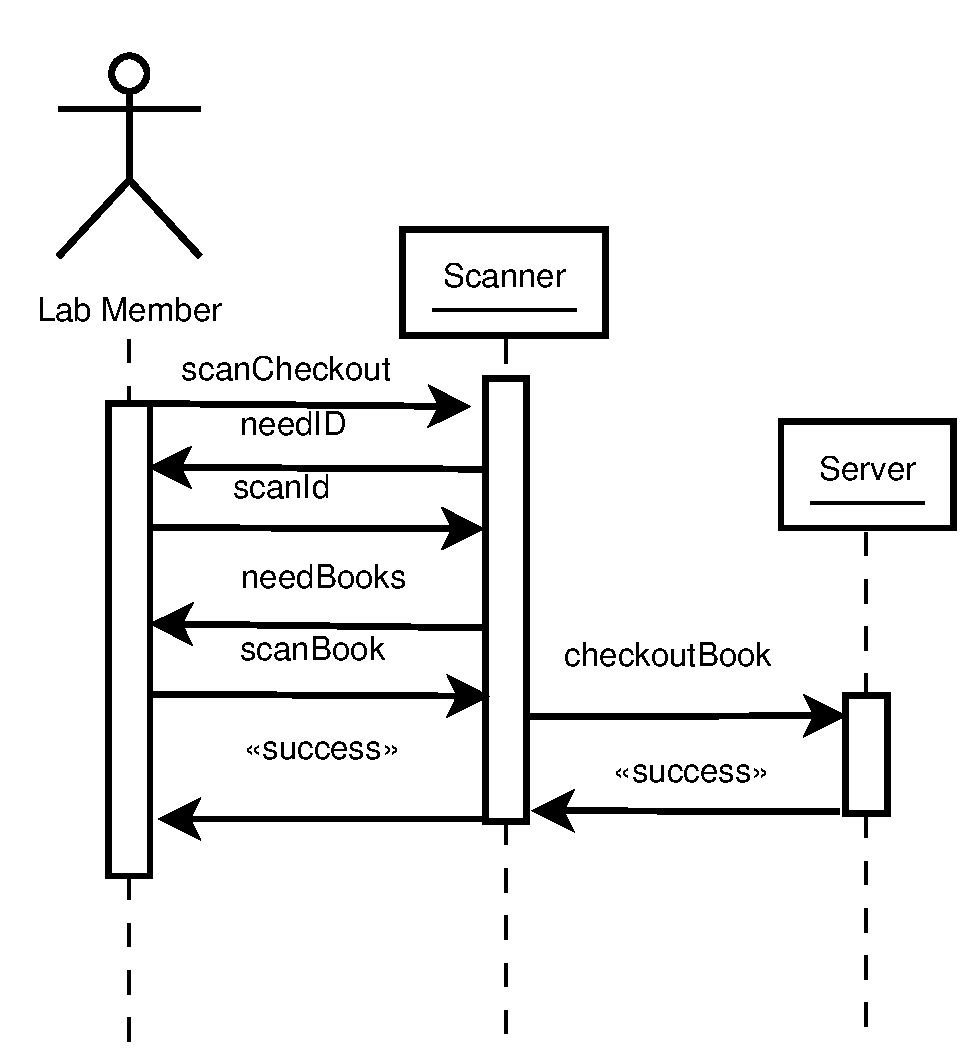
\includegraphics[width=0.9\textwidth]{Use_Case_1}
    \caption{Use Case 1 Sequence Diagram}
    \label{fig:usecase1_image}
\end{figure}

\begin{figure}[p]
    \centering
    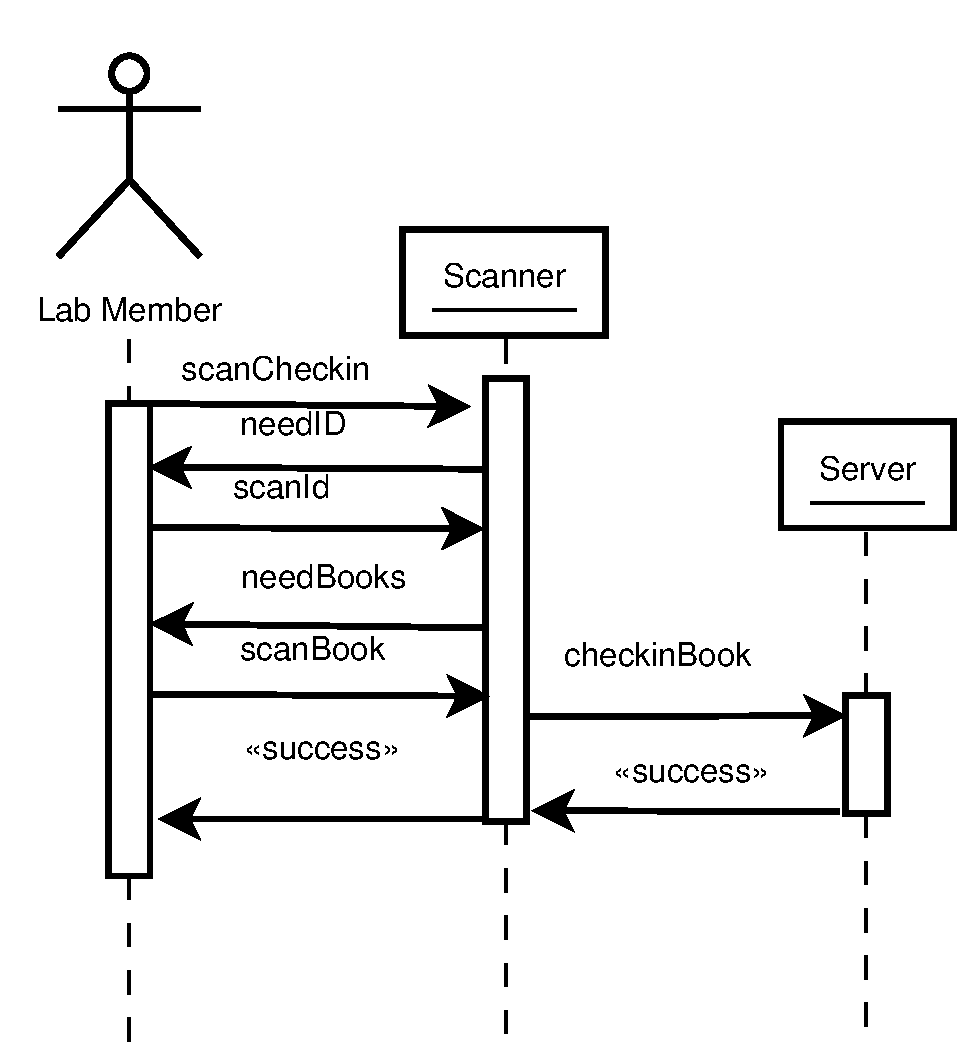
\includegraphics[width=0.9\textwidth]{Use_Case_2}
    \caption{Use Case 2 Sequence Diagram}
    \label{fig:usecase2_image}
\end{figure}

\begin{figure}[p]
    \centering
    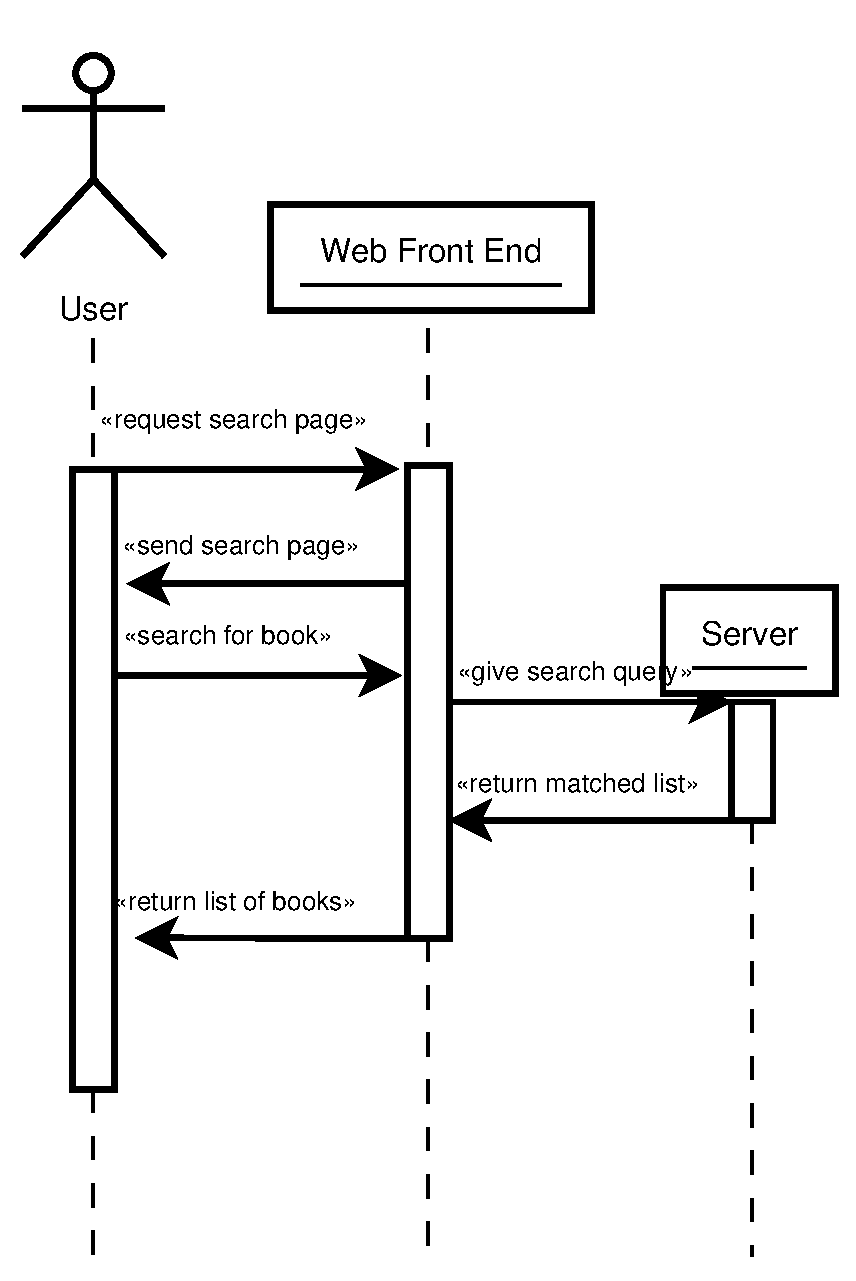
\includegraphics[width=0.9\textwidth]{Use_Case_3}
    \caption{Use Case 3 Sequence Diagram}
    \label{fig:usecase3_image}
\end{figure}

\begin{figure}[p]
    \centering
    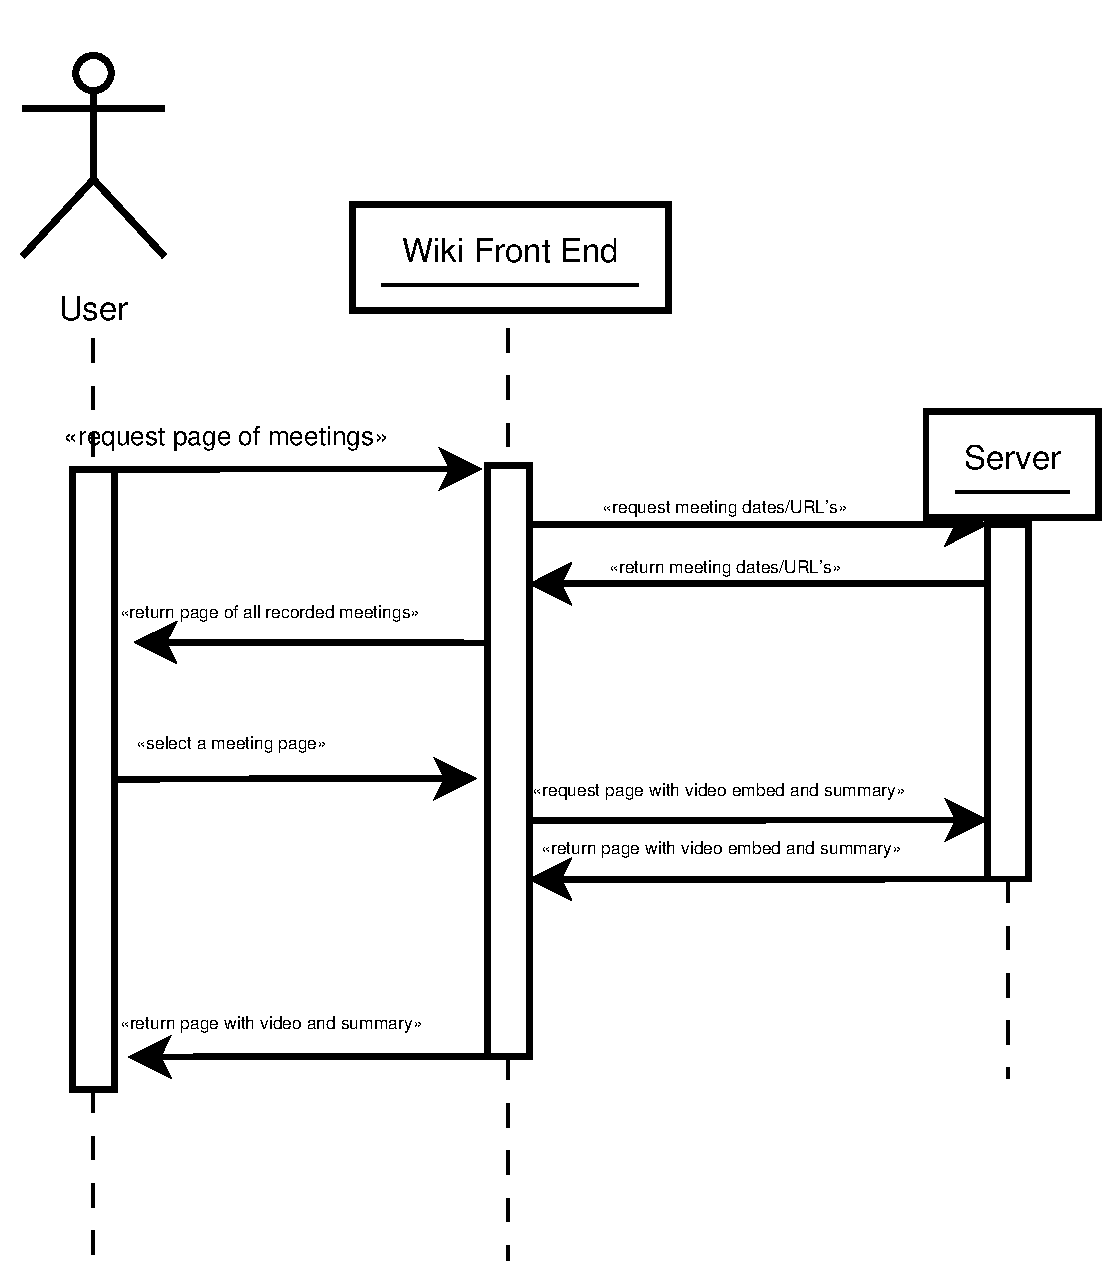
\includegraphics[width=0.9\textwidth]{Use_Case_4}
    \caption{Use Case 4 Sequence Diagram}
    \label{fig:usecase4_image}
\end{figure}

\begin{figure}[p]
    \centering
    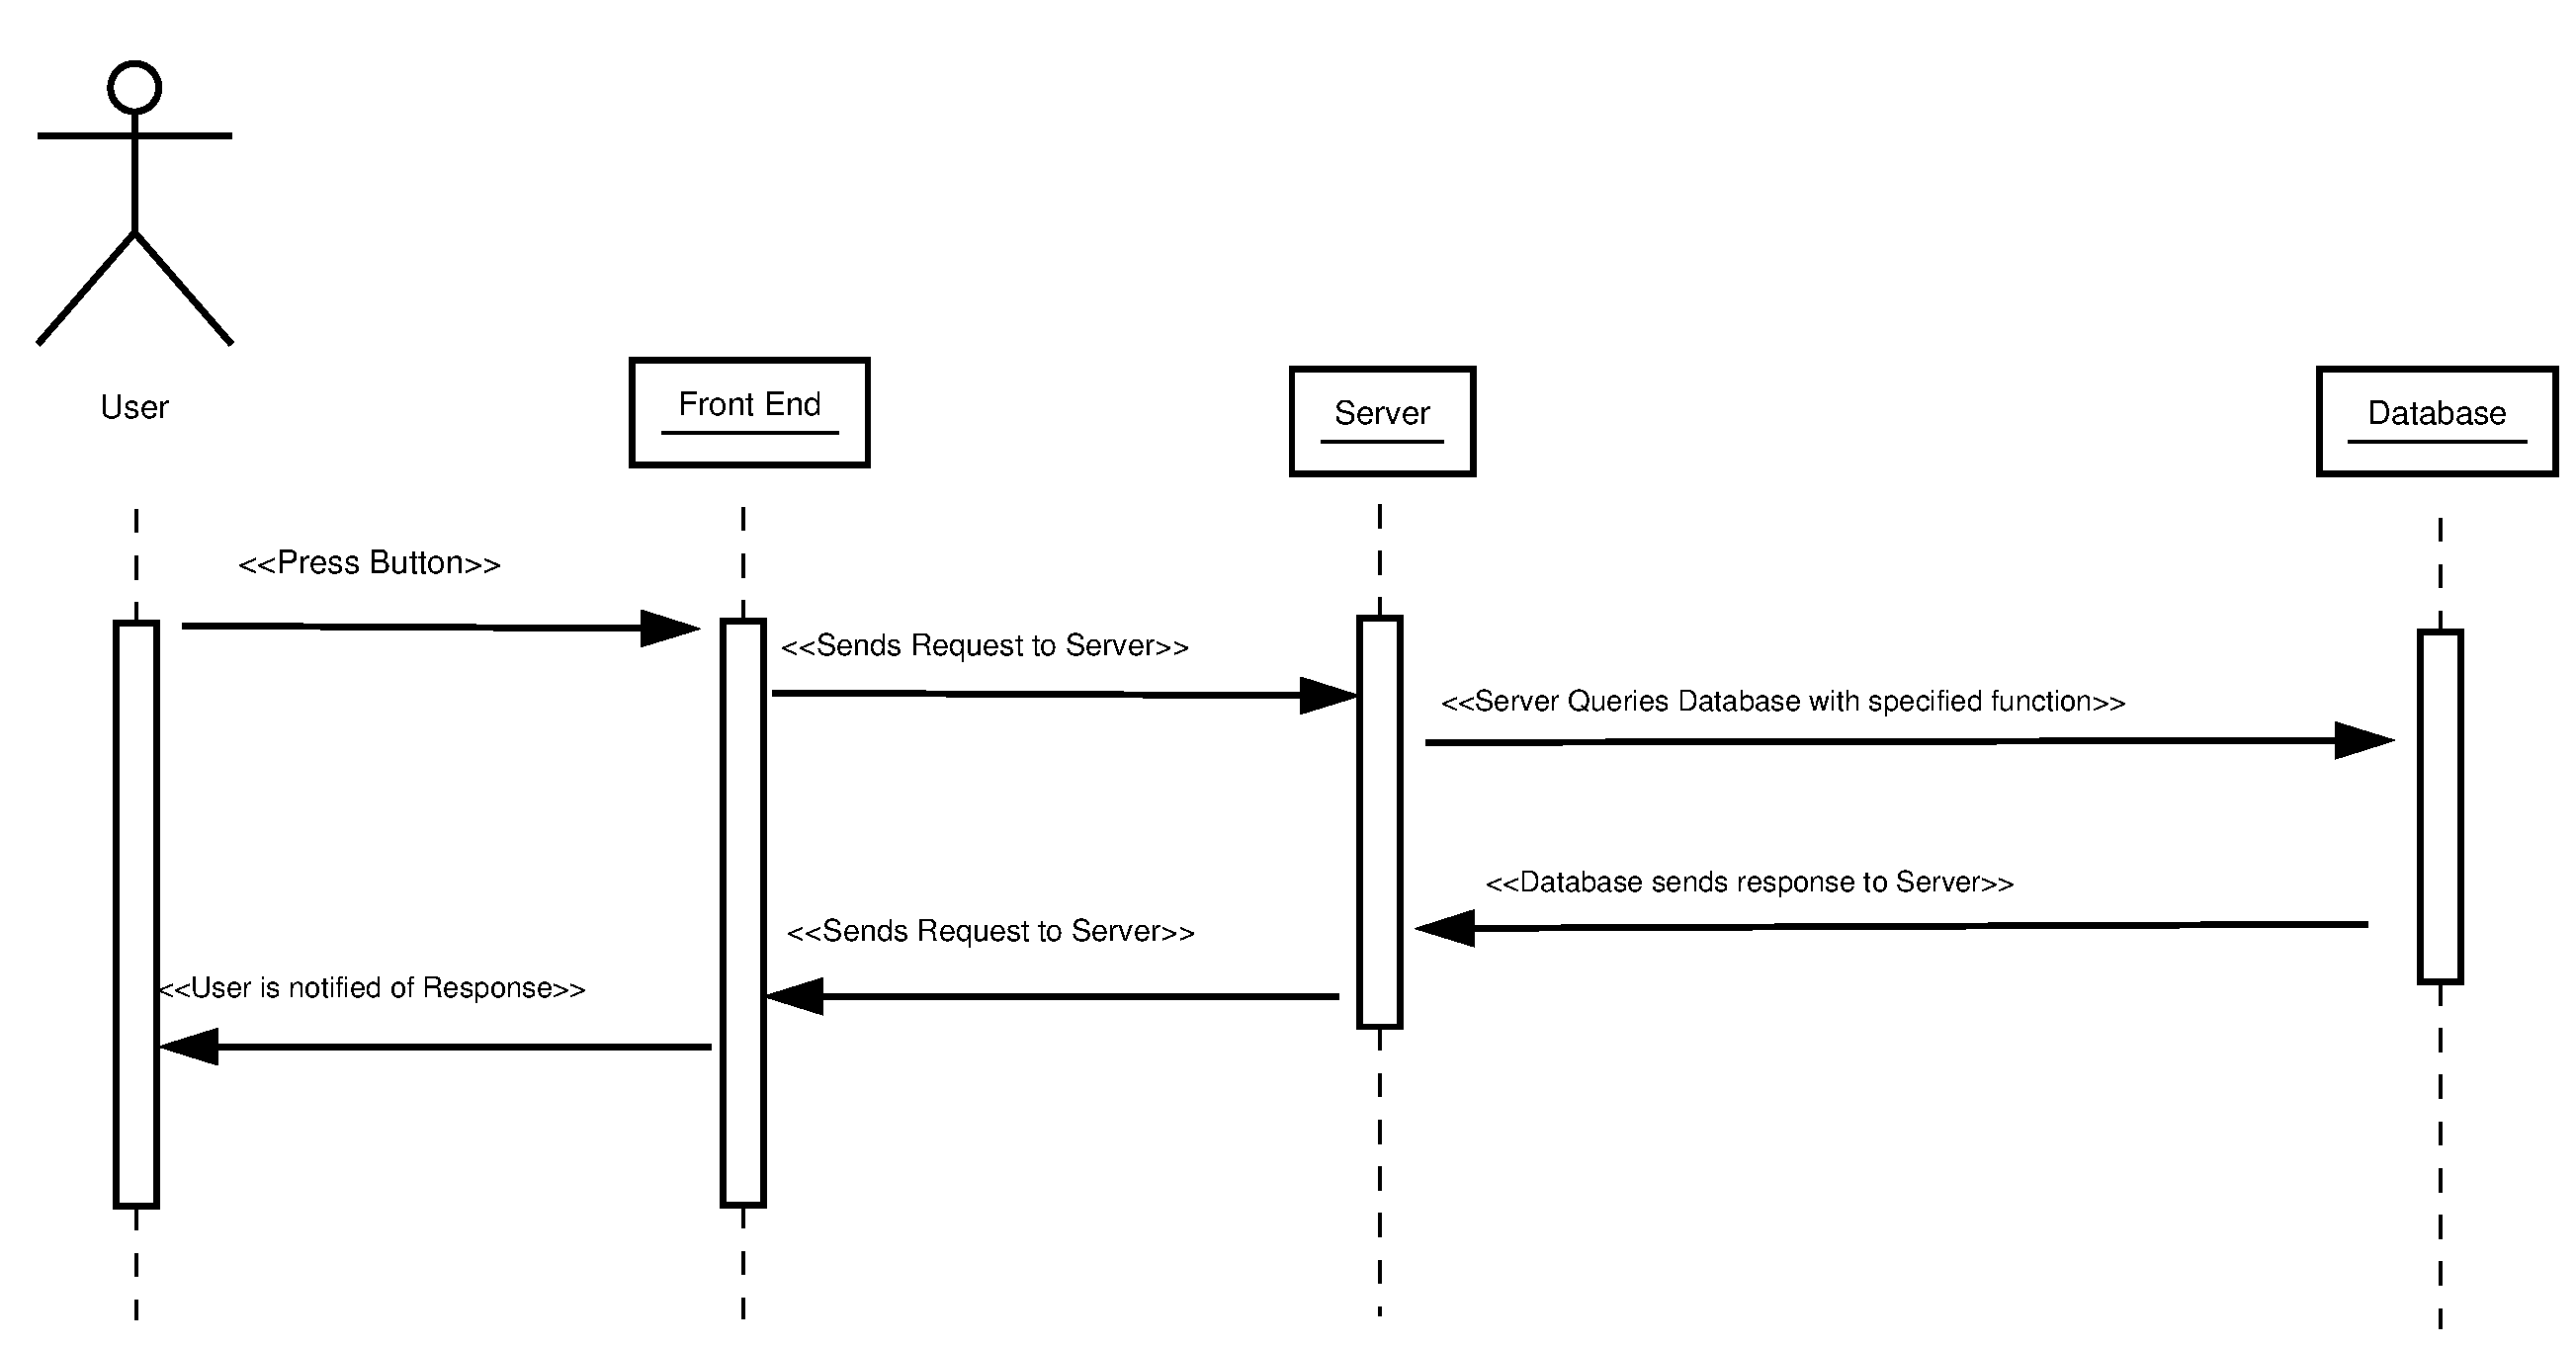
\includegraphics[width=0.9\textwidth]{Use_Case_5}
    \caption{Use Case 5 Sequence Diagram}
    \label{fig:usecase5_image}
\end{figure}

\begin{figure}[p]
    \centering
    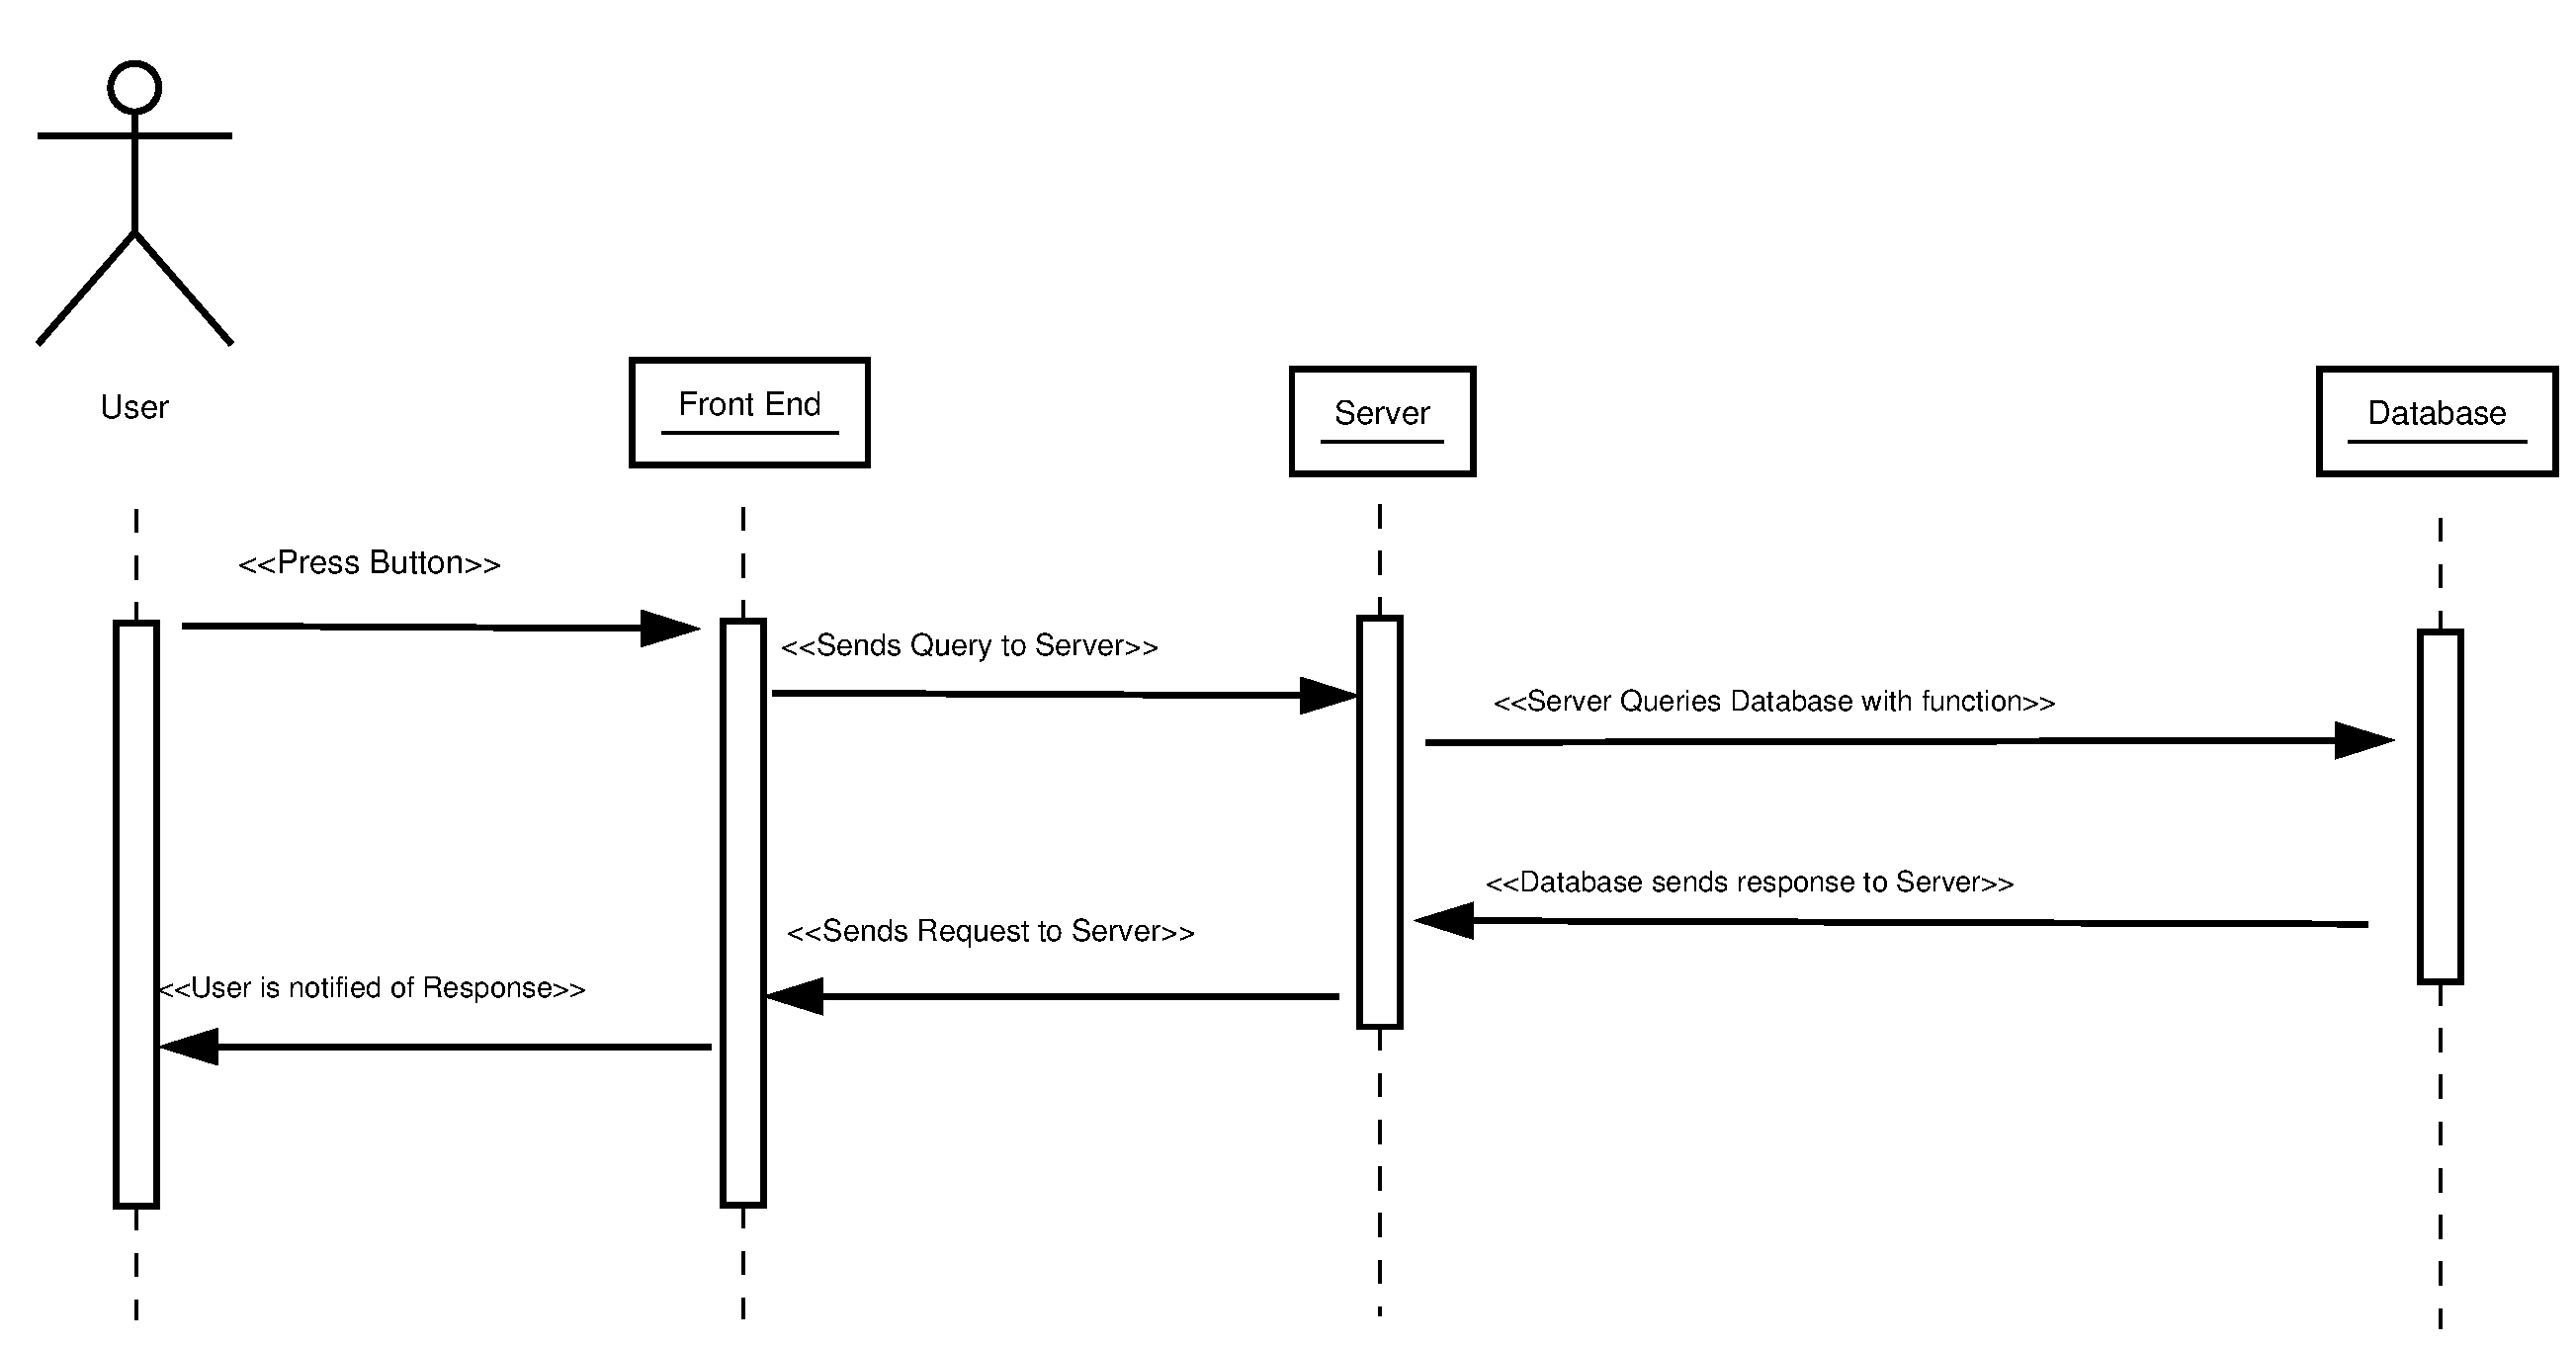
\includegraphics[width=0.9\textwidth]{Use_Case_6}
    \caption{Use Case 6 Sequence Diagram}
    \label{fig:usecase6_image}
\end{figure}

\end{document}
